\documentclass[]{article}
\usepackage{lmodern}
\usepackage{amssymb,amsmath}
\usepackage{ifxetex,ifluatex}
\usepackage{fixltx2e} % provides \textsubscript
\ifnum 0\ifxetex 1\fi\ifluatex 1\fi=0 % if pdftex
  \usepackage[T1]{fontenc}
  \usepackage[utf8]{inputenc}
\else % if luatex or xelatex
  \ifxetex
    \usepackage{mathspec}
  \else
    \usepackage{fontspec}
  \fi
  \defaultfontfeatures{Ligatures=TeX,Scale=MatchLowercase}
\fi
% use upquote if available, for straight quotes in verbatim environments
\IfFileExists{upquote.sty}{\usepackage{upquote}}{}
% use microtype if available
\IfFileExists{microtype.sty}{%
\usepackage{microtype}
\UseMicrotypeSet[protrusion]{basicmath} % disable protrusion for tt fonts
}{}
\usepackage[margin=1in]{geometry}
\usepackage{hyperref}
\hypersetup{unicode=true,
            pdftitle={MSc. Research Methods - Statistikteil Lösungen 2018},
            pdfauthor={Gian-Andrea Egeler},
            pdfborder={0 0 0},
            breaklinks=true}
\urlstyle{same}  % don't use monospace font for urls
\usepackage{color}
\usepackage{fancyvrb}
\newcommand{\VerbBar}{|}
\newcommand{\VERB}{\Verb[commandchars=\\\{\}]}
\DefineVerbatimEnvironment{Highlighting}{Verbatim}{commandchars=\\\{\}}
% Add ',fontsize=\small' for more characters per line
\usepackage{framed}
\definecolor{shadecolor}{RGB}{248,248,248}
\newenvironment{Shaded}{\begin{snugshade}}{\end{snugshade}}
\newcommand{\KeywordTok}[1]{\textcolor[rgb]{0.13,0.29,0.53}{\textbf{#1}}}
\newcommand{\DataTypeTok}[1]{\textcolor[rgb]{0.13,0.29,0.53}{#1}}
\newcommand{\DecValTok}[1]{\textcolor[rgb]{0.00,0.00,0.81}{#1}}
\newcommand{\BaseNTok}[1]{\textcolor[rgb]{0.00,0.00,0.81}{#1}}
\newcommand{\FloatTok}[1]{\textcolor[rgb]{0.00,0.00,0.81}{#1}}
\newcommand{\ConstantTok}[1]{\textcolor[rgb]{0.00,0.00,0.00}{#1}}
\newcommand{\CharTok}[1]{\textcolor[rgb]{0.31,0.60,0.02}{#1}}
\newcommand{\SpecialCharTok}[1]{\textcolor[rgb]{0.00,0.00,0.00}{#1}}
\newcommand{\StringTok}[1]{\textcolor[rgb]{0.31,0.60,0.02}{#1}}
\newcommand{\VerbatimStringTok}[1]{\textcolor[rgb]{0.31,0.60,0.02}{#1}}
\newcommand{\SpecialStringTok}[1]{\textcolor[rgb]{0.31,0.60,0.02}{#1}}
\newcommand{\ImportTok}[1]{#1}
\newcommand{\CommentTok}[1]{\textcolor[rgb]{0.56,0.35,0.01}{\textit{#1}}}
\newcommand{\DocumentationTok}[1]{\textcolor[rgb]{0.56,0.35,0.01}{\textbf{\textit{#1}}}}
\newcommand{\AnnotationTok}[1]{\textcolor[rgb]{0.56,0.35,0.01}{\textbf{\textit{#1}}}}
\newcommand{\CommentVarTok}[1]{\textcolor[rgb]{0.56,0.35,0.01}{\textbf{\textit{#1}}}}
\newcommand{\OtherTok}[1]{\textcolor[rgb]{0.56,0.35,0.01}{#1}}
\newcommand{\FunctionTok}[1]{\textcolor[rgb]{0.00,0.00,0.00}{#1}}
\newcommand{\VariableTok}[1]{\textcolor[rgb]{0.00,0.00,0.00}{#1}}
\newcommand{\ControlFlowTok}[1]{\textcolor[rgb]{0.13,0.29,0.53}{\textbf{#1}}}
\newcommand{\OperatorTok}[1]{\textcolor[rgb]{0.81,0.36,0.00}{\textbf{#1}}}
\newcommand{\BuiltInTok}[1]{#1}
\newcommand{\ExtensionTok}[1]{#1}
\newcommand{\PreprocessorTok}[1]{\textcolor[rgb]{0.56,0.35,0.01}{\textit{#1}}}
\newcommand{\AttributeTok}[1]{\textcolor[rgb]{0.77,0.63,0.00}{#1}}
\newcommand{\RegionMarkerTok}[1]{#1}
\newcommand{\InformationTok}[1]{\textcolor[rgb]{0.56,0.35,0.01}{\textbf{\textit{#1}}}}
\newcommand{\WarningTok}[1]{\textcolor[rgb]{0.56,0.35,0.01}{\textbf{\textit{#1}}}}
\newcommand{\AlertTok}[1]{\textcolor[rgb]{0.94,0.16,0.16}{#1}}
\newcommand{\ErrorTok}[1]{\textcolor[rgb]{0.64,0.00,0.00}{\textbf{#1}}}
\newcommand{\NormalTok}[1]{#1}
\usepackage{graphicx,grffile}
\makeatletter
\def\maxwidth{\ifdim\Gin@nat@width>\linewidth\linewidth\else\Gin@nat@width\fi}
\def\maxheight{\ifdim\Gin@nat@height>\textheight\textheight\else\Gin@nat@height\fi}
\makeatother
% Scale images if necessary, so that they will not overflow the page
% margins by default, and it is still possible to overwrite the defaults
% using explicit options in \includegraphics[width, height, ...]{}
\setkeys{Gin}{width=\maxwidth,height=\maxheight,keepaspectratio}
\IfFileExists{parskip.sty}{%
\usepackage{parskip}
}{% else
\setlength{\parindent}{0pt}
\setlength{\parskip}{6pt plus 2pt minus 1pt}
}
\setlength{\emergencystretch}{3em}  % prevent overfull lines
\providecommand{\tightlist}{%
  \setlength{\itemsep}{0pt}\setlength{\parskip}{0pt}}
\setcounter{secnumdepth}{0}
% Redefines (sub)paragraphs to behave more like sections
\ifx\paragraph\undefined\else
\let\oldparagraph\paragraph
\renewcommand{\paragraph}[1]{\oldparagraph{#1}\mbox{}}
\fi
\ifx\subparagraph\undefined\else
\let\oldsubparagraph\subparagraph
\renewcommand{\subparagraph}[1]{\oldsubparagraph{#1}\mbox{}}
\fi

%%% Use protect on footnotes to avoid problems with footnotes in titles
\let\rmarkdownfootnote\footnote%
\def\footnote{\protect\rmarkdownfootnote}

%%% Change title format to be more compact
\usepackage{titling}

% Create subtitle command for use in maketitle
\newcommand{\subtitle}[1]{
  \posttitle{
    \begin{center}\large#1\end{center}
    }
}

\setlength{\droptitle}{-2em}

  \title{MSc. Research Methods - Statistikteil Lösungen 2018}
    \pretitle{\vspace{\droptitle}\centering\huge}
  \posttitle{\par}
    \author{Gian-Andrea Egeler}
    \preauthor{\centering\large\emph}
  \postauthor{\par}
      \predate{\centering\large\emph}
  \postdate{\par}
    \date{November 2018}


\begin{document}
\maketitle

\subsubsection{Musterlösung Aufgabe 2.2: einfaktorielle
ANOVA}\label{musterlosung-aufgabe-2.2-einfaktorielle-anova}

\begin{Shaded}
\begin{Highlighting}[]
\NormalTok{df <-}\StringTok{ }\NormalTok{nova }\CommentTok{# klone den originaler Datensatz}

\CommentTok{# fasst die vier Inhalte der Gerichte zu drei Inhalten zusammen.}
\NormalTok{df}\OperatorTok{$}\NormalTok{label_content[}\KeywordTok{grep}\NormalTok{(}\StringTok{"Pflanzlich+"}\NormalTok{,df}\OperatorTok{$}\NormalTok{label_content)] <-}\StringTok{ "Vegetarisch"} 

\CommentTok{# gruppiert Daten nach Menü-Inhalt und Woche}
\NormalTok{df_ <-}\StringTok{ }\NormalTok{df }\OperatorTok
\StringTok{    }\KeywordTok{group_by}\NormalTok{(label_content, week) }\OperatorTok\StringTok{ }
\StringTok{    }\KeywordTok{summarise}\NormalTok{(}\DataTypeTok{tot_sold =} \KeywordTok{n}\NormalTok{()) }\OperatorTok
\StringTok{    }\KeywordTok{drop_na}\NormalTok{() }\CommentTok{# lasst die unbekannten Menü-Inhalte weg}

\CommentTok{# überprüft die Voraussetzungen für eine ANOVA}
\CommentTok{# Histogramm, sagt aber nicht viel aus}
\KeywordTok{ggplot}\NormalTok{(df_, }\KeywordTok{aes}\NormalTok{(}\DataTypeTok{x =}\NormalTok{ tot_sold, }\DataTypeTok{y =}\NormalTok{ ..count..)) }\OperatorTok{+}\StringTok{ }
\StringTok{  }\KeywordTok{geom_histogram}\NormalTok{() }\OperatorTok{+}\StringTok{ }
\StringTok{  }\KeywordTok{labs}\NormalTok{(}\DataTypeTok{x =} \StringTok{"}\CharTok{\textbackslash{}n}\StringTok{Anzahl verkaufte Gerichte pro Woche"}\NormalTok{, }\DataTypeTok{y =} \StringTok{"Häufigkeit}\CharTok{\textbackslash{}n}\StringTok{"}\NormalTok{) }\OperatorTok{+}
\StringTok{  }\NormalTok{mytheme }
\end{Highlighting}
\end{Shaded}

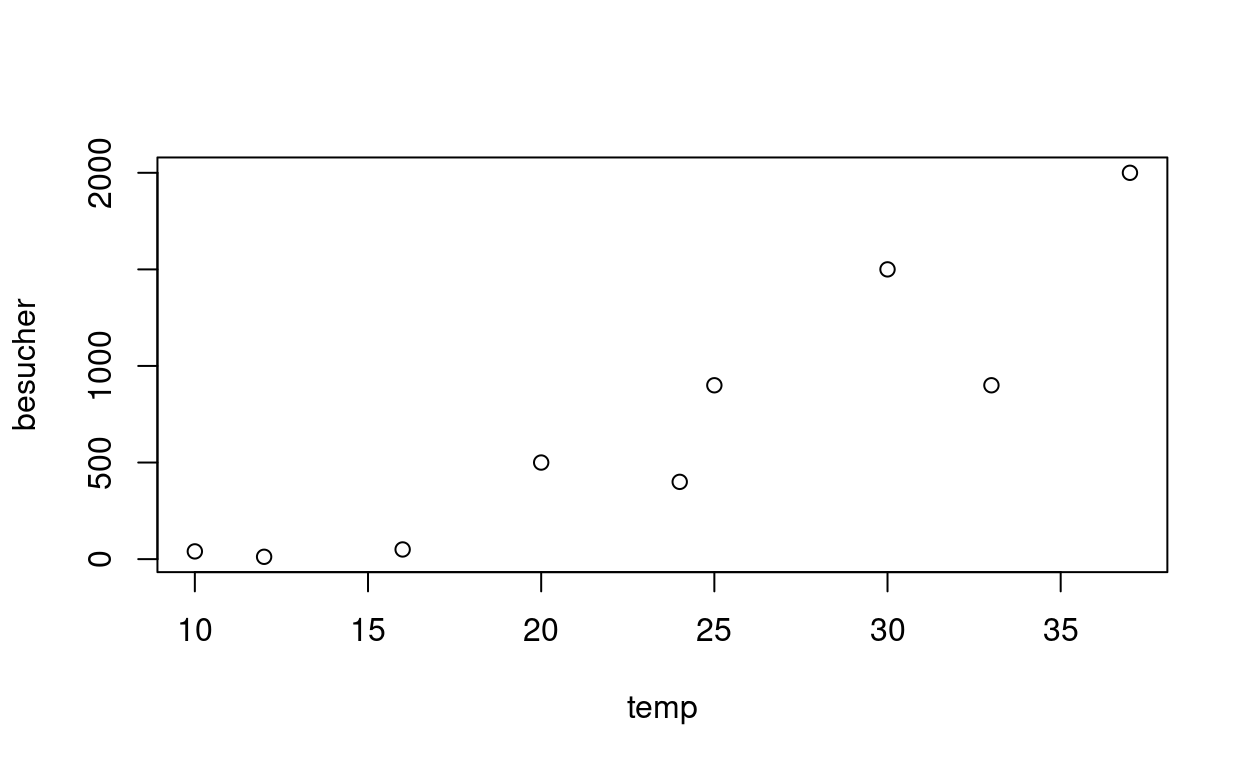
\includegraphics{Musterloesung_Statistik_2.2_files/figure-latex/unnamed-chunk-2-1.pdf}

\begin{Shaded}
\begin{Highlighting}[]
\CommentTok{# Boxplot}
\KeywordTok{ggplot}\NormalTok{(df_, }\KeywordTok{aes}\NormalTok{(}\DataTypeTok{x =}\NormalTok{ label_content, }\DataTypeTok{y=}\NormalTok{ tot_sold)) }\OperatorTok{+}
\StringTok{  }\KeywordTok{geom_boxplot}\NormalTok{(}\DataTypeTok{fill=}\StringTok{"white"}\NormalTok{, }\DataTypeTok{color =} \StringTok{"black"}\NormalTok{, }\DataTypeTok{size =} \DecValTok{1}\NormalTok{) }\OperatorTok{+}
\StringTok{  }\KeywordTok{labs}\NormalTok{(}\DataTypeTok{x =} \StringTok{"}\CharTok{\textbackslash{}n}\StringTok{Menü-Inhalt"}\NormalTok{, }\DataTypeTok{y =} \StringTok{"Anzahl verkaufte Gerichte pro Woche}\CharTok{\textbackslash{}n}\StringTok{"}\NormalTok{) }\OperatorTok{+}
\StringTok{  }\NormalTok{mytheme }\CommentTok{# klare Varianzheterogenität}
\end{Highlighting}
\end{Shaded}

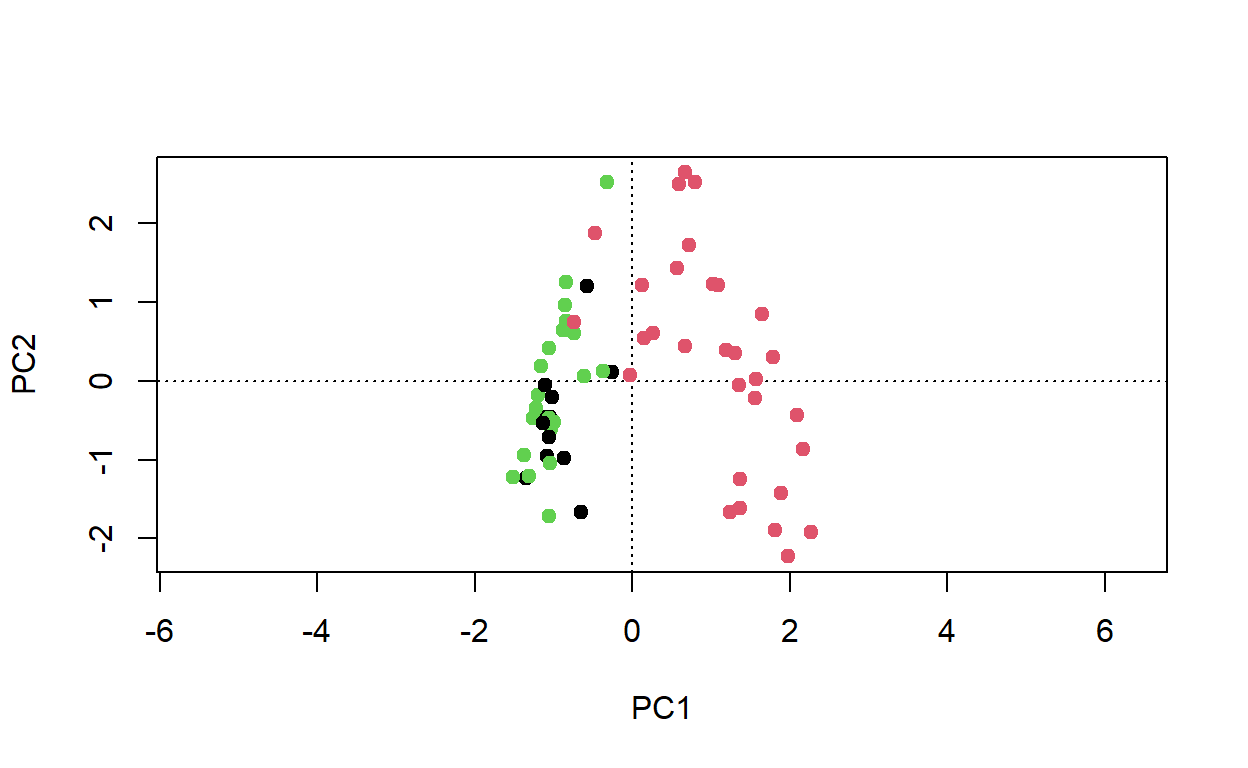
\includegraphics{Musterloesung_Statistik_2.2_files/figure-latex/unnamed-chunk-2-2.pdf}

\begin{Shaded}
\begin{Highlighting}[]
\CommentTok{# definiert das Modell}
\NormalTok{model <-}\StringTok{ }\KeywordTok{aov}\NormalTok{(tot_sold }\OperatorTok{~}\StringTok{ }\NormalTok{label_content, }\DataTypeTok{data =}\NormalTok{ df_)}

\KeywordTok{summary.lm}\NormalTok{(model)}
\end{Highlighting}
\end{Shaded}

\begin{verbatim}
## 
## Call:
## aov(formula = tot_sold ~ label_content, data = df_)
## 
## Residuals:
##      Min       1Q   Median       3Q      Max 
## -19.0000  -7.8750   0.3333   8.3750  23.0000 
## 
## Coefficients:
##                          Estimate Std. Error t value Pr(>|t|)    
## (Intercept)                25.667      5.193   4.943 0.000177 ***
## label_contentFleisch       68.333      7.344   9.305 1.28e-07 ***
## label_contentVegetarisch   38.833      7.344   5.288 9.11e-05 ***
## ---
## Signif. codes:  0 '***' 0.001 '**' 0.01 '*' 0.05 '.' 0.1 ' ' 1
## 
## Residual standard error: 12.72 on 15 degrees of freedom
## Multiple R-squared:  0.8531, Adjusted R-squared:  0.8335 
## F-statistic: 43.56 on 2 and 15 DF,  p-value: 5.653e-07
\end{verbatim}

\begin{Shaded}
\begin{Highlighting}[]
\KeywordTok{autoplot}\NormalTok{(model) }\OperatorTok{+}\StringTok{ }\NormalTok{mytheme }
\end{Highlighting}
\end{Shaded}

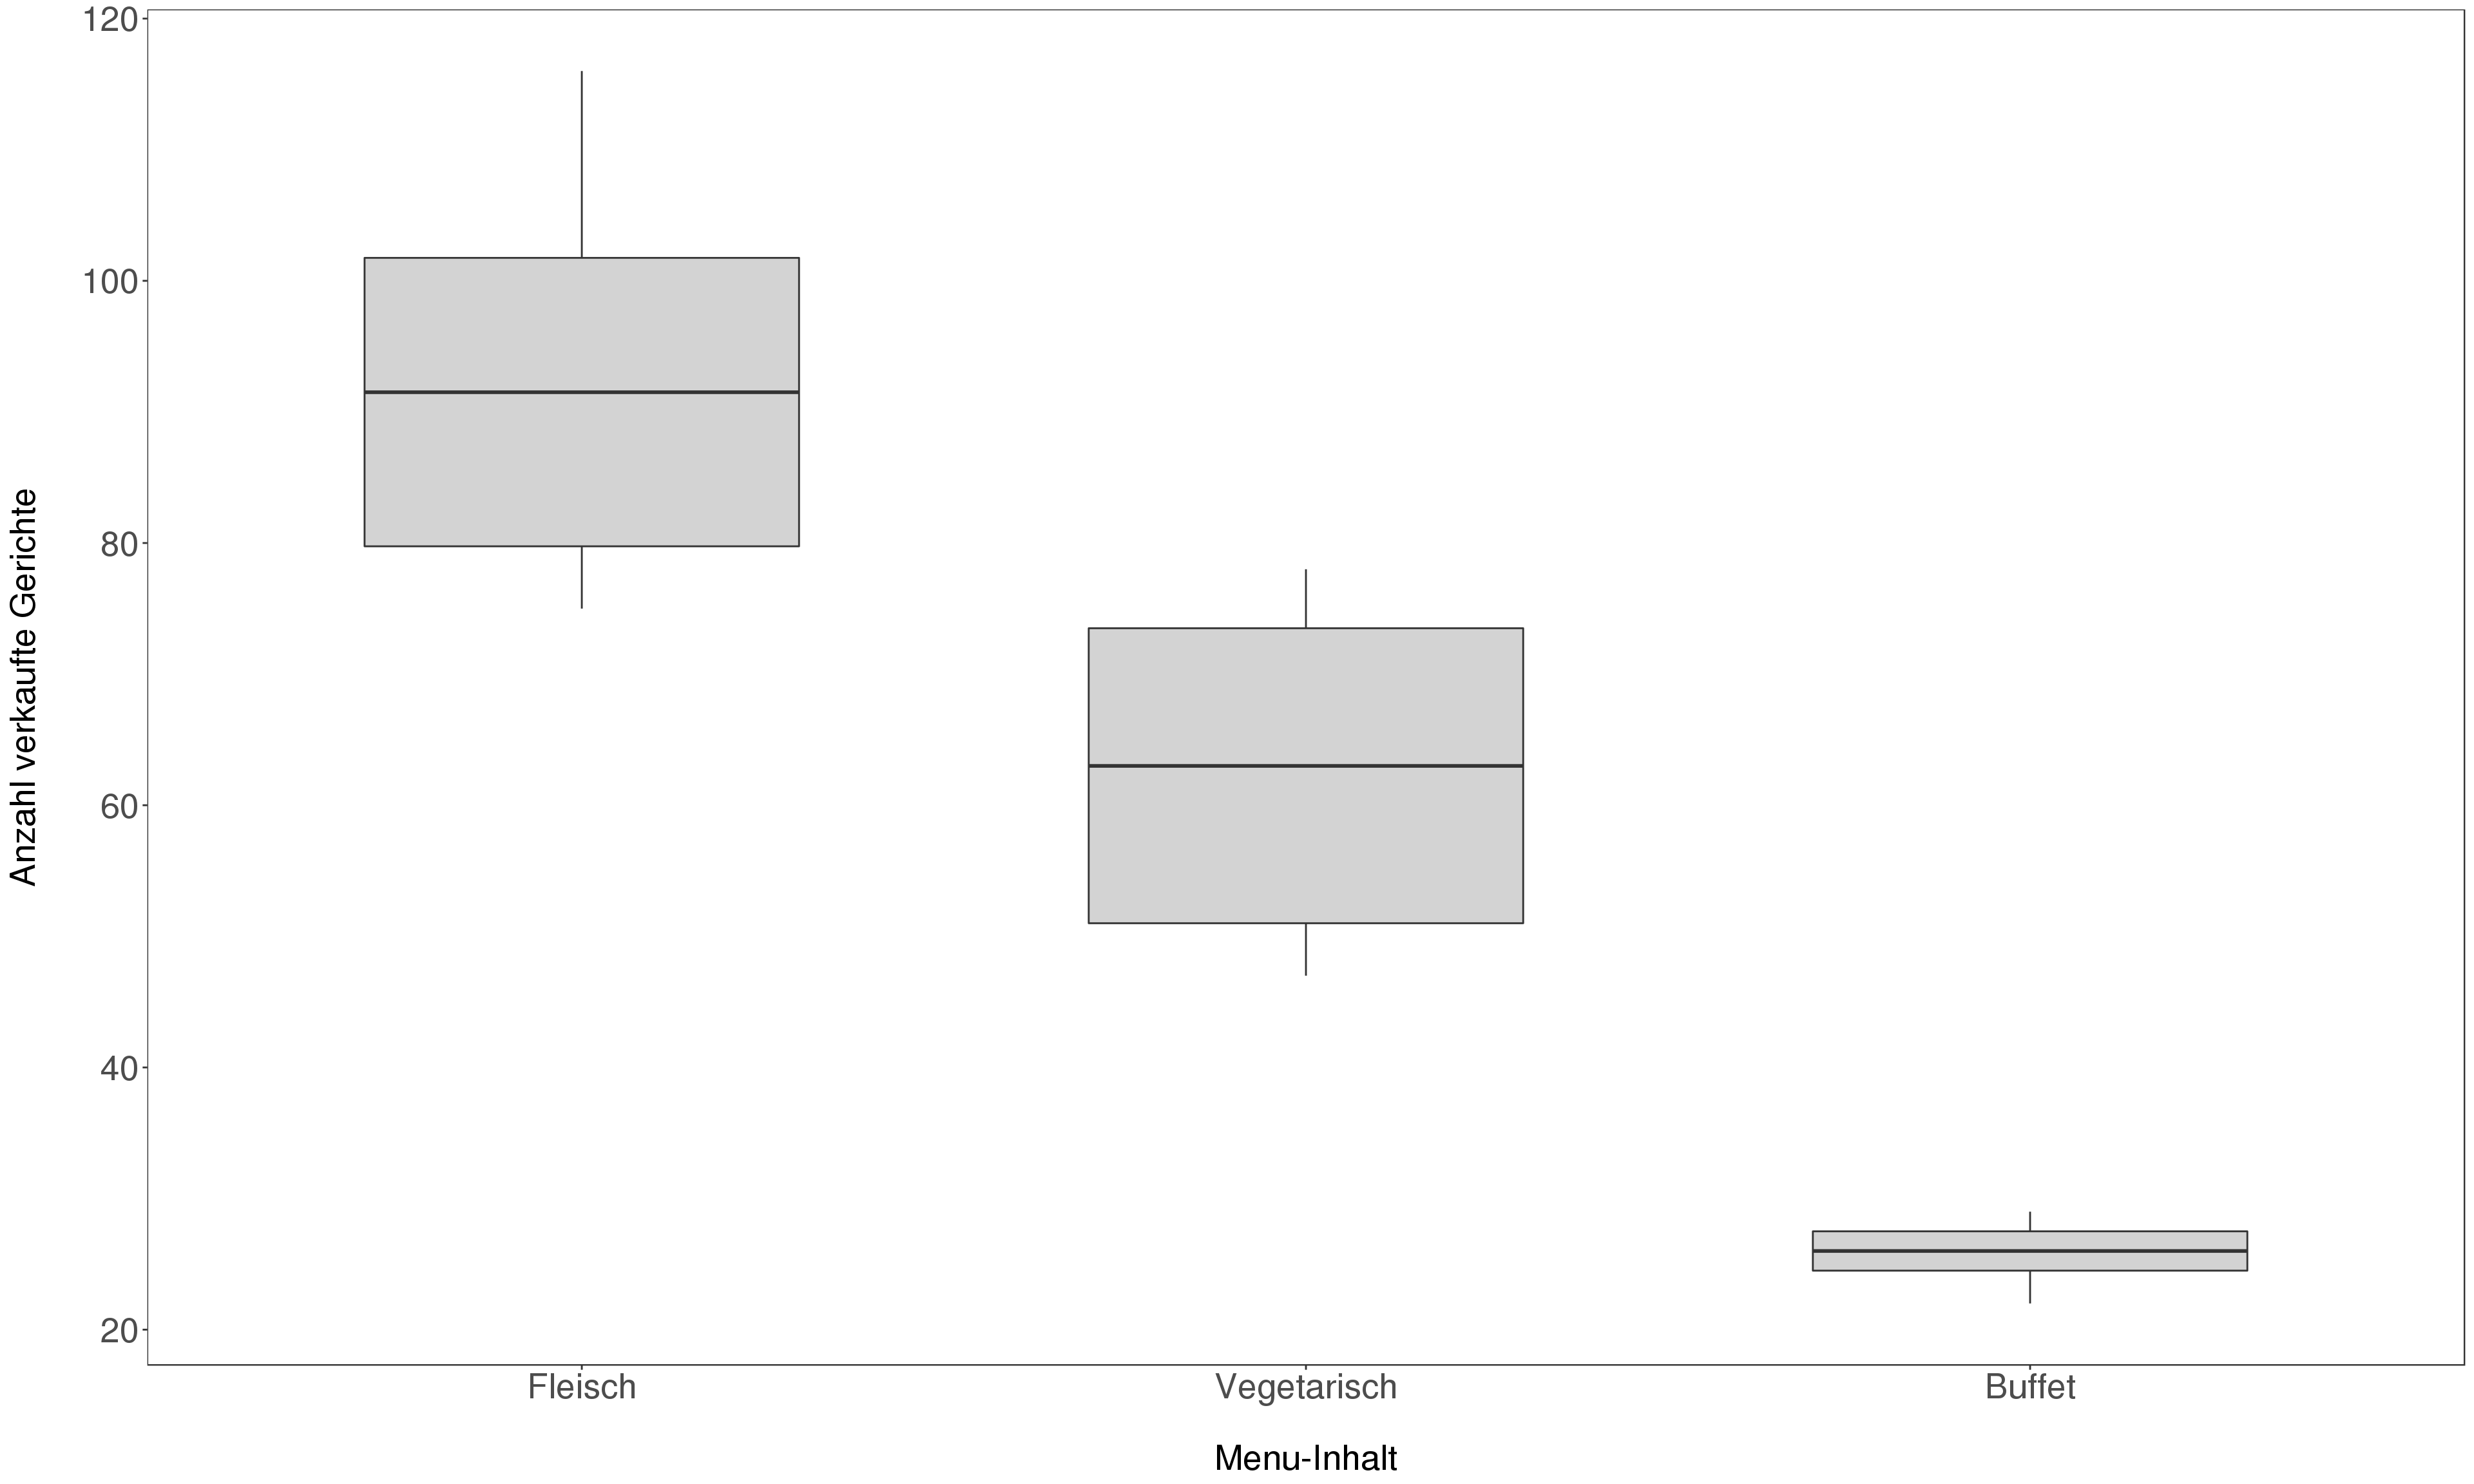
\includegraphics{Musterloesung_Statistik_2.2_files/figure-latex/unnamed-chunk-2-3.pdf}

Fazit: Inspektion der Modellvoraussetzung zeigt klare Verletzungen der
Homoskedastizität. Nächster Schritt Welch-Test.

\begin{Shaded}
\begin{Highlighting}[]
\CommentTok{# überprüft die Voraussetzungen des Welch-Test.}
\CommentTok{# Gibt es eine hohe Varianzheterogenität und }
\CommentTok{# ist die relative Verteilung der Residuen gegeben? }
\CommentTok{# In diesem Fall wäre ein Welch-Test passend}
\NormalTok{w_test <-}\StringTok{ }\KeywordTok{oneway.test}\NormalTok{(}\DataTypeTok{data=}\NormalTok{df_, tot_sold }\OperatorTok{~}\StringTok{ }\NormalTok{label_content, }\DataTypeTok{var.equal=}\NormalTok{F)}
\NormalTok{w_test}
\end{Highlighting}
\end{Shaded}

\begin{verbatim}
## 
##  One-way analysis of means (not assuming equal variances)
## 
## data:  tot_sold and label_content
## F = 64.997, num df = 2.0000, denom df = 6.9832, p-value =
## 3.067e-05
\end{verbatim}

\paragraph{Methoden}\label{methoden}

Ziel war es, die Unterschide in den Verkaufszahlen pro Menü-Inhalt
aufzuzeigen. Da die Kriteriumsvariable (Verkaufszahlen) metrisch und die
Prädiktorvariable kategorial sind, wurde eine einfaktorielle ANOVA
gerechnet. Die visuelle Inspektion der Voraussetzungen zeigte
insbesondere schwere Verletzungen der Homoskedastizität. Der Boxplot
bestätigt diesen Befund. Daher wurde in einem weiteren Schritt den
Welch-Test für ungleiche Varianzen gerechnet.

\paragraph{Ergebnisse}\label{ergebnisse}

Die Menü-Inhalte (Fleisch, Vegetarisch und Buffet) unterscheiden sich in
den Verkaufszahlen signifikant (\emph{F}(2,7) = 65, \emph{p} \textless{}
.001). Die Figure 1 zeigt die Verkaufszahlen pro Menü-Inhalt.

\begin{figure}
\centering
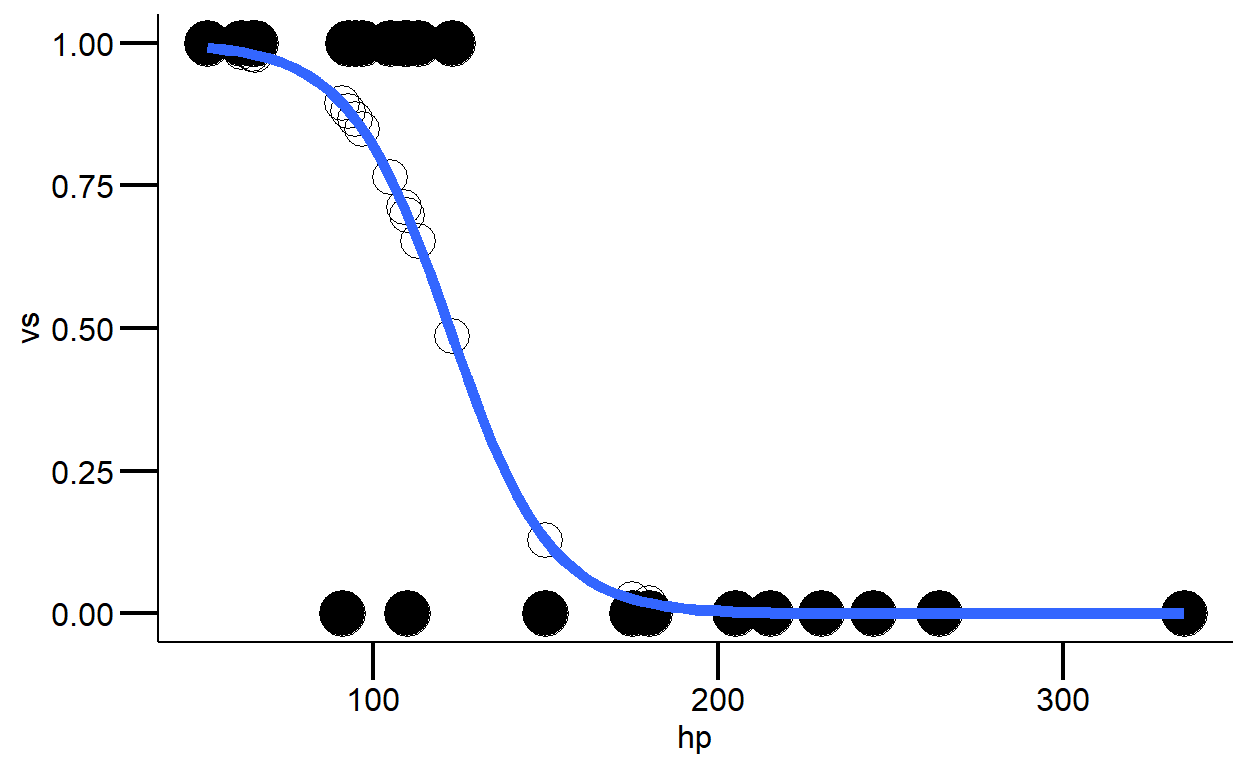
\includegraphics{Musterloesung_Statistik_2.2_files/figure-latex/unnamed-chunk-4-1.pdf}
\caption{Die wöchentlichen Verkaufzahlen unterscheiden sich je nach
Menü-Inhalt stark.}
\end{figure}


\end{document}
